%-----------------------------------LICENSE------------------------------------%
%   This file is part of Mathematics-and-Physics.                              %
%                                                                              %
%   Mathematics-and-Physics is free software: you can redistribute it and/or   %
%   modify it it under the terms of the GNU General Public License as          %
%   published by the Free Software Foundation, either version 3 of the         %
%   License, or (at your option) any later version.                            %
%                                                                              %
%   Mathematics-and-Physics is distributed in the hope that it will be useful, %
%   but WITHOUT ANY WARRANTY; without even the implied warranty of             %
%   MERCHANTABILITY or FITNESS FOR A PARTICULAR PURPOSE.  See the              %
%   GNU General Public License for more details.                               %
%                                                                              %
%   You should have received a copy of the GNU General Public License along    %
%   with Mathematics-and-Physics.  If not, see <https://www.gnu.org/licenses/>.%
%------------------------------------------------------------------------------%

%   Use the standalone class for displaying the tikz image on a small PDF.
\documentclass[crop, tikz]{standalone}

%   Import the tikz package to use for the drawing.
\usepackage{tikz}

%   Begin the document.
\begin{document}

    %   Draw the figure.
    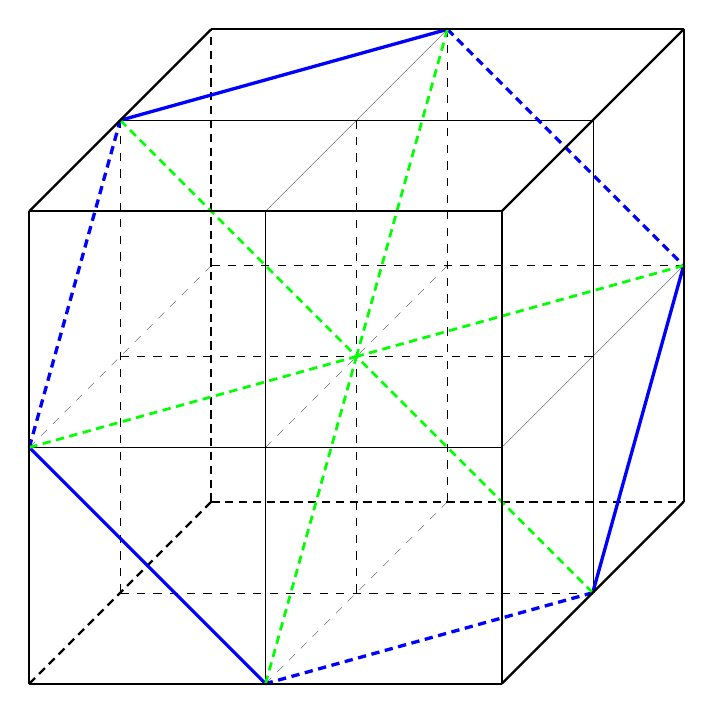
\begin{tikzpicture}

        % Lots of coordinates.
        \coordinate (O) at (0, 0, 0);
        \coordinate (x) at (6, 0, 0);
        \coordinate (y) at (0, 6, 0);
        \coordinate (z) at (0, 0, 6);
        \coordinate (xy) at (6, 6, 0);
        \coordinate (xz) at (6, 0, 6);
        \coordinate (yz) at (0, 6, 6);
        \coordinate (xyz) at (6, 6, 6);
        \coordinate (MID) at (3, 3, 3);
        \coordinate (a1) at (3, 0, 6);
        \coordinate (a2) at (3, 6, 6);
        \coordinate (a3) at (0, 3, 6);
        \coordinate (a4) at (6, 3, 6);
        \coordinate (b1) at (0, 0, 3);
        \coordinate (b2) at (6, 0, 3);
        \coordinate (b3) at (a1);
        \coordinate (b4) at (3, 0, 0);
        \coordinate (c1) at (b2);
        \coordinate (c2) at (6, 6, 3);
        \coordinate (c3) at (a4);
        \coordinate (c4) at (6, 3, 0);
        \coordinate (d1) at (0, 6, 3);
        \coordinate (d2) at (c2);
        \coordinate (d3) at (a2);
        \coordinate (d4) at (3, 6, 0);
        \coordinate (e1) at (a3);
        \coordinate (e2) at (0, 3, 0);
        \coordinate (e3) at (b1);
        \coordinate (e4) at (d1);
        \coordinate (f1) at (e2);
        \coordinate (f2) at (c4);
        \coordinate (f3) at (b4);
        \coordinate (f4) at (d4);
        \coordinate (A) at (3, 3, 6);
        \coordinate (B) at (3, 0, 3);
        \coordinate (C) at (6, 3, 3);
        \coordinate (D) at (3, 6, 3);
        \coordinate (E) at (0, 3, 3);
        \coordinate (F) at (3, 3, 0);

        % Draw the back of the cube.
        \begin{scope}[thick]
            \draw[densely dashed] (O) to (x);
            \draw[densely dashed] (O) to (y);
            \draw[densely dashed] (O) to (z);
        \end{scope}

        % Some dashed lines inside the cube.
        \begin{scope}[line width=0.1pt]
            \draw (a1) to (a2);
            \draw (a3) to (a4);
            \draw[dashed] (b1) to (b2);
            \draw[dashed] (b3) to (b4);
            \draw (c1) to (c2);
            \draw (c3) to (c4);
            \draw (d1) to (d2);
            \draw (d3) to (d4);
            \draw[dashed] (e1) to (e2);
            \draw[dashed] (e3) to (e4);
            \draw[dashed] (f1) to (f2);
            \draw[dashed] (f3) to (f4);
            \draw[dashed] (A) to (MID);
            \draw[dashed] (B) to (MID);
            \draw[dashed] (C) to (MID);
            \draw[dashed] (D) to (MID);
            \draw[dashed] (E) to (MID);
            \draw[dashed] (F) to (MID);
        \end{scope}

        % Draw the hexagon.
        \begin{scope}[very thick, blue]
            \draw(a1) to (a3);
            \draw[densely dashed] (a3) to (d1);
            \draw (d1) to (d4);
            \draw[densely dashed] (d4) to (c4);
            \draw (c4) to (b2);
            \draw[densely dashed] (b2) to (a1);
        \end{scope}

        % Connect vertices to center of cube.
        \begin{scope}[densely dashed, green, line width=1pt]
            \draw (a1) to (MID);
            \draw (a3) to (MID);
            \draw (d1) to (MID);
            \draw (c4) to (MID);
            \draw (d4) to (MID);
            \draw (b2) to (MID);
        \end{scope}

        % Draw the front of the cube.
        \begin{scope}[thick]
            \draw (x) to (xy);
            \draw (y) to (xy);
            \draw (x) to (xz);
            \draw (z) to (xz);
            \draw (y) to (yz);
            \draw (z) to (yz);
            \draw (xy) to (xyz);
            \draw (yz) to (xyz);
            \draw (xz) to (xyz);
        \end{scope}
    \end{tikzpicture}
\end{document}
